\section{Gleichstrommaschine im Umrichterbetrieb}

Diese Section behandelt die \textbf{Gleichstrommaschine} als Last und Antrieb im Zusammenspiel mit
\textbf{Gleichrichtern} und \textbf{Gleichstromstellern}.
Sie ist zentral für die Analyse von \textbf{Drehzahl}, \textbf{Drehmoment}, \textbf{Stabilität} und
für das Verständnis der \textbf{Kennlinien $M$--$n$} sowie des \textbf{Quadrantenbetriebs}.

\smallskip

\textbf{Zielbild:}
\begin{itemize}
    \item Grundgleichungen der Gleichstrommaschine kennen (elektrisch und mechanisch)
    \item Zusammenhang zwischen Spannung, Strom, Drehzahl und Drehmoment verstehen
    \item Einfluss der Ankerspannung und des Erregerflusses auf die Kennlinie analysieren
    \item Arbeitspunkt bestimmen und Stabilität beurteilen
    \item Betrieb mit 1Q-, 2Q- und 4Q-Stellern (Motor/Generator) einordnen
\end{itemize}

\subsection*{Konvention für Maschinenkonstanten}

Zur Vereinheitlichung der Notation wird im Folgenden definiert:

\[
\boxed{k\Phi \;\equiv\; \Psi}
\]

mit:
\begin{itemize}
    \item $\Phi$: Erregerfluss,
    \item $k$: Maschinenkonstante,
    \item $\Psi$: zusammengefasste Flusskonstante der Maschine.
\end{itemize}

Damit gilt einheitlich:
\[
E_i = \Psi \, \omega,
\qquad
M = \Psi \, i_a.
\]


% =========================================================
\subsection{Grundaufbau und Ersatzschaltbild}

\begin{center}
    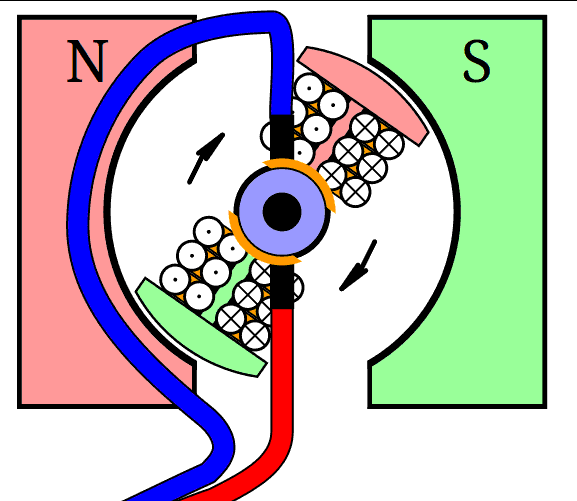
\includegraphics[width=0.85\linewidth]{images/Grundaufbau_gleistrommaschiene.png}
\end{center}

\subsubsection{Vereinfachtes Ersatzschaltbild}

\begin{center}
    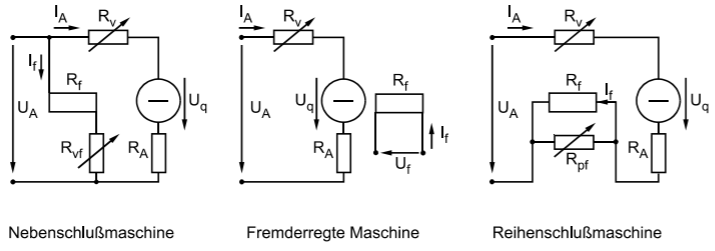
\includegraphics[width=0.85\linewidth]{images/gleichstrommasciene.png}
\end{center}

\paragraph{Elemente und Variablen}
\begin{itemize}
    \item $u_a(t)$: Ankerspannung (Ausgangsspannung des Umrichters bzw. Stellers),
    \item $i_a(t)$: Ankerstrom,
    \item $R_a$: Ankerwiderstand,
    \item $L_a$: Ankerinduktivität,
    \item $E_i(t)$: induzierte Gegenspannung (Gegen-EMK),
    \item $\omega(t)$: mechanische Winkelgeschwindigkeit,
    \item $n(t)$: Drehzahl in $\mathrm{min^{-1}}$,
    \item $M(t)$: elektromagnetisches Drehmoment.
\end{itemize}

Zusammenhang zwischen Drehzahl und Winkelgeschwindigkeit:
\[
\boxed{\omega = 2\pi \frac{n}{60}}
\]

% =========================================================
\subsection{Maschinenkonstanten und Grundzusammenhänge}

Zur einheitlichen Schreibweise wird die Maschinenkonstante $k\Phi$ verwendet.

\paragraph{Gegen-EMK}
\[
\boxed{E_i = k\Phi\,\omega}
\]

\paragraph{Drehmoment}
\[
\boxed{M = k\Phi\,i_a}
\]

mit:
\begin{itemize}
    \item $\Phi$: Erregerfluss (bzw. proportional dazu),
    \item $k$: Maschinenkonstante (Konstruktionsparameter),
    \item $k\Phi$: resultierende Konstante aus Maschine und Erregung.
\end{itemize}

\crd{\textrightarrow\ In den Grundgleichungen koppelt $k\Phi$ den elektrischen und mechanischen Teil.}

% =========================================================
\subsection{Grundgleichungen der Gleichstrommaschine}

\subsubsection{Elektrische Gleichung}

\[
\boxed{u_a(t) = R_a\, i_a(t) + L_a\, \frac{di_a(t)}{dt} + E_i(t)}
\]

Einsetzen von $E_i=k\Phi\omega$:
\[
\boxed{u_a(t) = R_a i_a(t) + L_a\frac{di_a(t)}{dt} + k\Phi\,\omega(t)}
\]

\subsubsection{Mechanische Gleichung}

\[
\boxed{J\frac{d\omega(t)}{dt} = M(t) - M_L(t) - B\,\omega(t)}
\]

mit:
\begin{itemize}
    \item $J$: Trägheitsmoment,
    \item $M_L$: Lastmoment,
    \item $B$: viskoser Reibungskoeffizient.
\end{itemize}

\subsubsection{Leistungsbeziehungen}

Elektrische Leistung:
\[
\boxed{P_{el}(t)=u_a(t)\,i_a(t)}
\]

Mechanische Leistung:
\[
\boxed{P_{mech}(t)=M(t)\,\omega(t)}
\]

Ideal (ohne Verluste) gilt näherungsweise:
\[
\boxed{P_{el}\approx P_{mech}}
\]

\crd{\textrightarrow\ Drehmoment wird direkt durch den Strom bestimmt: $M=k\Phi i_a$.}

% =========================================================
\subsection{Stationärer Betrieb}

Im stationären Betrieb gilt:
\[
\frac{di_a}{dt}=0,
\qquad
\frac{d\omega}{dt}=0
\]

Damit reduziert sich die elektrische Gleichung zu:
\[
\boxed{u_a = R_a i_a + k\Phi\,\omega}
\]

Auflösen nach der Drehzahl:
\[
\boxed{\omega=\frac{u_a-R_a i_a}{k\Phi}}
\]

\subsubsection{Strom als Funktion von Spannung und Drehzahl}

Aus $u_a=R_a i_a+k\Phi\omega$ folgt:
\[
\boxed{i_a=\frac{u_a-k\Phi\omega}{R_a}}
\]

Daraus Drehmoment als Funktion von $u_a$ und $\omega$:
\[
\boxed{M=k\Phi\,i_a=\frac{k\Phi}{R_a}\left(u_a-k\Phi\omega\right)}
\]

Interpretation:
\begin{itemize}
    \item $u_a\uparrow \Rightarrow \omega\uparrow$ (bei gleicher Last),
    \item $M_L\uparrow \Rightarrow i_a\uparrow \Rightarrow \omega\downarrow$.
\end{itemize}

% =========================================================
\subsection{Spezialfall: Leerlaufbetrieb}

Leerlauf bedeutet: sehr kleines Lastmoment $M_L \approx 0$ und damit sehr kleiner Ankerstrom $i_a \approx 0$.
Im idealen Leerlauf (ohne Reibung) folgt aus $M = i_a \Psi$ direkt $i_a \approx 0$.
Damit gilt stationär aus $u_a = R_a i_a + \omega \Psi$ näherungsweise:

\[
\boxed{i_{a,0} \approx 0}
\]
\[
\boxed{\omega_0 \approx \frac{u_a}{\Psi}}
\]

Mit Reibung $B$ ergibt sich im stationären Betrieb näherungsweise:
\[
M \approx B\omega
\quad\Rightarrow\quad
i_a \approx \frac{B\omega}{\Psi}
\]
und damit:
\[
\boxed{u_a \approx R_a\frac{B\omega}{\Psi} + \omega\Psi}
\]

mit:
\begin{itemize}
\item $M_L$: Lastmoment,
\item $B$: Reibungskoeffizient,
\item $i_{a,0}$: Leerlaufstrom,
\item $\omega_0$: Leerlaufdrehzahl.
\end{itemize}
\subsection{Spezialfall: Blockierfall (gesperrter Rotor)}

Im Blockierfall ist der Rotor mechanisch gesperrt:
\[
\boxed{\omega = 0}
\]

Damit ist die Gegen-EMK null:
\[
\boxed{E_i = \omega\Psi = 0}
\]

Die elektrische Gleichung reduziert sich im stationären Fall ($di_a/dt=0$) zu:
\[
\boxed{u_a = R_a i_a}
\quad\Rightarrow\quad
\boxed{i_{a,\mathrm{block}} = \frac{u_a}{R_a}}
\]

Das Blockiermoment ergibt sich aus $M=i_a\Psi$:
\[
\boxed{M_{\mathrm{block}} = i_{a,\mathrm{block}}\,\Psi = \frac{u_a\Psi}{R_a}}
\]

Konsequenz:
\begin{itemize}
\item Der Blockierstrom ist sehr hoch und nur durch $R_a$ begrenzt.
\item Thermische Überlast ist wahrscheinlich $\Rightarrow$ Strombegrenzung erforderlich.
\end{itemize}

mit:
\begin{itemize}
\item $i_{a,\mathrm{block}}$: Blockierstrom,
\item $M_{\mathrm{block}}$: Blockiermoment.
\end{itemize}
\subsection{M--n-Kennlinie (Drehmoment--Drehzahl-Kennlinie)}

Mit
\[
M=k\Phi i_a,
\qquad
u_a=R_a i_a+k\Phi\omega
\]

Elimination von $i_a$:
\[
i_a=\frac{M}{k\Phi}
\]

Einsetzen in $u_a=R_a i_a+k\Phi\omega$:
\[
u_a=R_a\frac{M}{k\Phi}+k\Phi\omega
\]

Auflösen nach $\omega$:
\[
\boxed{\omega=\frac{u_a}{k\Phi}-\frac{R_a}{(k\Phi)^2}M}
\]

Dies ist eine \textbf{lineare Kennlinie}.

\subsubsection{Kennwerte}

Leerlaufdrehzahl (bei $M\approx 0$):
\[
\boxed{\omega_0=\frac{u_a}{k\Phi}}
\]

Kurzschlussmoment (bei $\omega=0$):
\[
\boxed{M_K=\frac{u_a\,k\Phi}{R_a}}
\]

\subsubsection{Normierte Kennlinie}

Normierte Grössen:
\[
\boxed{\omega^*=\frac{\omega}{\omega_0}},
\qquad
\boxed{M^*=\frac{M}{M_K}}
\]

Damit folgt:
\[
\boxed{\omega^*=1-M^*}
\]

\crd{\textrightarrow\ Normiert ist die M--n-Kennlinie eine Gerade von $(M^*=0,\omega^*=1)$ nach $(M^*=1,\omega^*=0)$.}

% =========================================================
\subsection{Dynamisches Modell der Gleichstrommaschine}

\paragraph{Elektrisch}
\[
\boxed{u_a(t)=R_a i_a(t)+L_a\frac{di_a(t)}{dt}+k\Phi\,\omega(t)}
\]

\paragraph{Mechanisch}
\[
\boxed{J\frac{d\omega(t)}{dt}=k\Phi\,i_a(t)-M_L(t)-B\,\omega(t)}
\]

Das System ist ein gekoppeltes elektrisches--mechanisches System.
Die Kopplung erfolgt über $k\Phi$.

% =========================================================
\subsection{Einfluss der Ankerspannung $u_a$}

Die Kennlinie
\[
\omega=\frac{u_a}{k\Phi}-\frac{R_a}{(k\Phi)^2}M
\]
zeigt:

\begin{itemize}
    \item Erhöhung von $u_a$ verschiebt die Kennlinie parallel nach oben,
    \item die Steigung $-\frac{R_a}{(k\Phi)^2}$ bleibt konstant.
\end{itemize}

\crd{\textrightarrow\ Spannungsregelung $\Rightarrow$ Drehzahlregelung (bei konstantem Fluss).}

% =========================================================
\subsection{Einfluss des Erregerflusses}

Mit variablem Fluss (Feldschwächung) gilt:
\[
\omega_0=\frac{u_a}{k\Phi},
\qquad
M=k\Phi i_a
\]

\begin{itemize}
    \item $\Phi\downarrow \Rightarrow \omega_0\uparrow$ (höhere Drehzahl möglich),
    \item $\Phi\downarrow \Rightarrow M$ pro Strom sinkt (geringere Drehmomentfähigkeit),
    \item Feldschwächung dient der Erweiterung des Drehzahlbereichs.
\end{itemize}

% =========================================================
\subsection{Arbeitspunkt und Stabilität}

Der Arbeitspunkt ist der Schnittpunkt von Motorkennlinie und Lastkennlinie.

\begin{itemize}
    \item Motorkennlinie: $\omega_M(M)$,
    \item Lastkennlinie: $\omega_L(M)$.
\end{itemize}

\subsubsection{Stabilitätskriterium}

\[
\boxed{\frac{d\omega_M}{dM} < \frac{d\omega_L}{dM}\;\Rightarrow\;\text{stabil}}
\]

\crd{\textrightarrow\ Bei falscher Steigung entsteht instabiler Betrieb (Arbeitspunkt wandert).}

% =========================================================
\subsection{Betrieb in den vier Quadranten}

In Kombination mit 1Q-, 2Q- und 4Q-Gleichstromstellern kann die Gleichstrommaschine
in unterschiedlichen Quadranten betrieben werden.

\paragraph{Leistungskriterium}
\[
\boxed{P=u_a i_a=M\omega}
\]

\begin{itemize}
\item $P>0$: Motorbetrieb (Energie von Quelle zur Maschine),
\item $P<0$: Generatorbetrieb (Rekuperation zur Quelle).
\end{itemize}

\paragraph{Quadrant I: Motorbetrieb vorwärts}
\[
\boxed{u_a>0,\; i_a>0,\; \omega>0,\; M>0}
\]

\paragraph{Quadrant II: Generatorbetrieb vorwärts (Bremsbetrieb)}
\[
\boxed{u_a<0,\; i_a>0,\; \omega>0,\; M<0}
\]

\paragraph{Quadrant III: Motorbetrieb rückwärts}
\[
\boxed{u_a<0,\; i_a<0,\; \omega<0,\; M<0}
\]

\paragraph{Quadrant IV: Generatorbetrieb rückwärts}
\[
\boxed{u_a>0,\; i_a<0,\; \omega<0,\; M>0}
\]

\crd{\textrightarrow\ 4Q-Steller ist erforderlich, wenn Spannungs- und Stromumkehr benötigt werden.}

% =========================================================
\subsection{Zusammenhang mit Umrichter und Steller}

Die Ankerspannung $u_a$ wird durch den vorgeschalteten Umrichter bestimmt.

\subsubsection{Gleichstromsteller (Chopper, CCM)}

\[
\boxed{u_a=u_d=d\,U_{DC}}
\]

mit:
\begin{itemize}
\item $d$: Tastgrad,
\item $U_{DC}$: Eingangsgleichspannung des Stellers.
\end{itemize}

\subsubsection{Gesteuerter Gleichrichter (z.B. B2C/B6C)}

\[
\boxed{u_a=\overline{u_d}=K\,U\cos\alpha}
\]

mit:
\begin{itemize}
\item $\alpha$: Zündwinkel,
\item $U$: zugehörige Netz-Effektivspannung (je nach Topologie),
\item $K$: Topologiekonstante (z.B. $K=\frac{2\sqrt{2}}{\pi}$ für B2C, $K=\frac{3\sqrt{2}}{\pi}$ für B6C).
\end{itemize}

Konsequenz:
\begin{itemize}
    \item Drehzahl wird direkt über $d$ oder $\alpha$ beeinflusst,
    \item Drehmoment wird direkt über $i_a$ beeinflusst.
\end{itemize}

% =========================================================
\subsection{Schnellentscheidungshilfen für die Gleichstrommaschine}

Diese Merksätze erlauben eine schnelle qualitative Beurteilung in Prüfungsaufgaben.

\paragraph{Grundgleichungen}

\[
\boxed{u_a = R_a i_a + k\Phi \omega}
\]
\[
\boxed{M = k\Phi i_a}
\]

\paragraph{Einfluss der Ankerspannung $u_a$}

\begin{itemize}
\item $u_a \uparrow \Rightarrow \omega \uparrow$ (bei gleicher Last),
\item $u_a \downarrow \Rightarrow \omega \downarrow$,
\item $u_a = 0 \Rightarrow \omega \approx 0$ (Stillstand, idealisiert).
\end{itemize}

\paragraph{Einfluss des Lastmoments $M_L$}

\begin{itemize}
\item $M_L \uparrow \Rightarrow i_a \uparrow \Rightarrow \omega \downarrow$,
\item $M_L \downarrow \Rightarrow i_a \downarrow \Rightarrow \omega \uparrow$.
\end{itemize}

\paragraph{Einfluss des Erregerflusses $\Phi$}

\begin{itemize}
\item $\Phi \uparrow \Rightarrow \omega_0 \downarrow$,
\item $\Phi \downarrow \Rightarrow \omega_0 \uparrow$,
\item $\Phi \downarrow \Rightarrow M_{\max} \downarrow$ (bei gleichem Stromlimit).
\end{itemize}

\paragraph{Motoranlauf}

Beim Anlauf gilt:
\[
\omega=0 \Rightarrow E_i=k\Phi\omega=0
\]

Damit:
\[
\boxed{i_{a,0}=\frac{u_a}{R_a}}
\]

Anlaufmoment:
\[
\boxed{M_0=k\Phi i_{a,0}}
\]

Konsequenzen:
\begin{itemize}
\item Sehr hoher Anlaufstrom,
\item Strombegrenzung oder Regelung notwendig,
\item Drehmoment beim Anlauf maximal (strombegrenzt).
\end{itemize}

\crd{\textrightarrow\ Diese Merksätze erlauben schnelle qualitative Entscheidungen ohne Rechnung.}

% =========================================================
\subsection{Typische Merksätze (Prüfungskern)}

\begin{itemize}
    \item $E_i = k\Phi \omega$
    \item $M = k\Phi i_a$
    \item $\omega = \dfrac{u_a - R_a i_a}{k\Phi}$
    \item $i_a = \dfrac{u_a - k\Phi \omega}{R_a}$
    \item M--n-Kennlinie ist linear.
    \item $P=u_a i_a = M\omega$ und Vorzeichen entscheidet Motor/Generator.
\end{itemize}

% =========================================================
\subsection{Typische Fehlerquellen}

\begin{itemize}
    \item Gegen-EMK $E_i$ vergessen oder falsches Vorzeichen.
    \item Drehmoment fälschlich aus Spannung statt aus Strom bestimmt.
    \item $\omega$ in $\mathrm{rad/s}$ und $n$ in $\mathrm{min^{-1}}$ verwechselt.
    \item Stabilitätskriterium über Steigungen falsch interpretiert.
    \item Feldschwächung nicht berücksichtigt (Fluss als konstant angenommen).
\end{itemize}

% =========================================================
\subsection{Minimal-Checkliste für Aufgaben}

\begin{enumerate}
    \item Gegebenes Stellglied identifizieren $\Rightarrow$ $u_a$ bestimmen (z.B. $u_a=dU_{DC}$ oder $u_a=K U\cos\alpha$).
    \item Gegen-EMK ansetzen: $E_i=k\Phi\omega$.
    \item Stationär: $i_a = \dfrac{u_a-k\Phi\omega}{R_a}$ berechnen.
    \item Drehmoment: $M=k\Phi i_a$ bestimmen.
    \item Arbeitspunkt: Schnitt Motor--Last (Kennlinien) bestimmen.
    \item Vorzeichen von $P=u_ai_a$ prüfen $\Rightarrow$ Motor/Generator.
    \item Stabilität qualitativ über Steigungen beurteilen.
\end{enumerate}

% =========================================================
\subsection{Allgemeine Motorgrundgleichungen (Übersicht)}

Elektrisch:
\[
\boxed{u = R i + L\frac{di}{dt} + E}
\]

Gegen-EMK:
\[
\boxed{E = k_e \omega = k_1 n}
\]

Drehmoment:
\[
\boxed{M = k_m i}
\]

Mechanisch:
\[
\boxed{J\frac{d\omega}{dt} = M - M_L - B\omega}
\]

Leistung:
\[
\boxed{P_{el}=u i,\qquad P_{mech}=M\omega}
\]
